\documentclass[conference]{IEEEtran}
\usepackage[T1]{fontenc}
\usepackage[utf8]{inputenc}
\usepackage[spanish,es-tabla,es-nodecimaldot,es-noshorthands]{babel}
\usepackage{amsmath,amssymb}
\usepackage{graphicx}
\usepackage{booktabs}
\usepackage{multirow}
\usepackage{cite}
\usepackage{xurl}
\usepackage{xcolor}
\usepackage{listings}
\usepackage{tikz}
\usetikzlibrary{positioning,arrows.meta}

% Items the team must confirm before submitting (remove when done)
\newcommand{\pendiente}[1]{\textcolor{red}{[PENDIENTE: #1]}}

\lstset{basicstyle=\ttfamily\scriptsize, breaklines=true, frame=single, columns=fullflexible,
        keywordstyle=\bfseries, showstringspaces=false}

\graphicspath{{figures/}}

\begin{document}

\title{Construcción de una Ontología Gastronómica para Recomendar Platos según Restricciones Alimentarias y Alergias, Trujillo, 2026}

\author{
\IEEEauthorblockN{Avila Sanchez Ulises Medardo}
\IEEEauthorblockA{Escuela de Informática\\Universidad Nacional de Trujillo\\muavilas@unitru.edu.pe}
\and
\IEEEauthorblockN{Quispe Ishuiza Cristopher}
\IEEEauthorblockA{Escuela de Informática\\Universidad Nacional de Trujillo\\cquispei@unitru.edu.pe}
\and
\IEEEauthorblockN{Reyes Casana Valentino}
\IEEEauthorblockA{Escuela de Informática\\Universidad Nacional de Trujillo\\jvreyesc@unitru.edu.pe}
}

\maketitle

\begin{abstract}
Los comensales con alergias, restricciones alimentarias u objetivos de control de peso deciden con información incompleta, porque la composición de los platos rara vez está estructurada. Este trabajo construye una ontología OWL 2 de la cocina peruana, con énfasis en Trujillo, que sirve de base a un sistema de recomendación basado en conocimiento. Se elaboró un conjunto de datos de 100 platos (50 de la costa, 30 de la sierra y 20 de la selva) y 146 ingredientes normalizados con 59 sinónimos regionales; se modeló la ontología, se pobló automáticamente, se verificó su consistencia con el razonador HermiT y se desplegó, junto con su motor de reglas, en Apache Jena Fuseki sobre la plataforma en la nube Render. En una evaluación comparativa con 30 consultas SPARQL (3000 pares consulta--plato), la versión refinada del motor elevó la Precision media de 0,668 a 0,918, el Recall de 0,909 a 0,987 y la medida F$_1$ de 0,735 a 0,942, diferencias significativas según la prueba de Wilcoxon ($p<0{,}05$). Las consultas sobre alérgenos y dietas alcanzaron Precision 1,0, mientras que los errores residuales se concentran en los perfiles nutricionales cualitativos.
\end{abstract}

\begin{IEEEkeywords}
ontologías, OWL, SPARQL, sistemas basados en conocimiento, recomendación de alimentos, alérgenos, cocina peruana.
\end{IEEEkeywords}

\section{Introducción}

\subsection{Realidad Problemática}

La alimentación es uno de los principales determinantes de la salud de las personas y, por ello, su regulación y comunicación se apoyan en guías, bases de datos y vocabularios de alcance internacional. Sin embargo, esa información dista de ser homogénea. Un análisis basado en procesamiento de lenguaje natural sobre las guías alimentarias de 98 países mostró diferencias semánticas consistentes entre grupos de países según su nivel de ingreso, incluso al comunicar las recomendaciones para un mismo grupo de alimentos como los lácteos \cite{bertini2026}. La heterogeneidad alcanza también a los datos alimentarios, cuya integración sigue siendo difícil por la diversidad de fuentes y formatos \cite{bindt2026}. Desde la investigación en nutrición se ha planteado, además, la necesidad de bases de composición de alimentos completas y accesibles, así como de una ontología común que permita reportar y comparar la evidencia de forma reproducible \cite{maruvada2020}.

Esta falta de estructura tiene consecuencias clínicas cuando la persona que se alimenta debe evitar determinados componentes. En la evaluación de la seguridad de ingredientes de fórmulas infantiles, un panel de expertos incluyó la alergia y las enfermedades atópicas entre los desenlaces clínicos estándar, lo que respalda considerar la respuesta inmunitaria a los componentes de un alimento como un criterio de seguridad relevante \cite{callahan2022}. En una persona alérgica, la exposición a un alérgeno, aun en cantidades muy pequeñas por contaminación cruzada durante la preparación, puede desencadenar reacciones que van desde manifestaciones cutáneas y digestivas hasta la anafilaxia. Las restricciones alimentarias tampoco se agotan en la alergia: en la disfagia, por ejemplo, evitar consistencias percibidas como inseguras conduce con frecuencia a desnutrición y a una ingesta desequilibrada de nutrientes \cite{spoladore2024}. En ambos casos, decidir qué plato es apropiado exige razonar de forma simultánea sobre ingredientes, procesos de preparación y condición del consumidor.

En el ámbito de la restauración el problema se agrava, porque la información que el comensal necesita (qué ingredientes contiene un plato y con qué otros productos comparte superficies y utensilios) rara vez está estructurada: suele residir en cartas en texto libre, en la memoria del personal o en recetas no estandarizadas. Sistemas recientes intentan cerrar esa brecha extrayendo información de etiquetas nutricionales mediante reconocimiento óptico de caracteres, recuperación semántica y modelos de lenguaje para emparejar alérgenos y emitir alertas personalizadas \cite{prasad2026}. Esta tendencia se inscribe en un uso creciente de modelos de lenguaje de gran tamaño (LLM) para el razonamiento orientado a la decisión en el sector agroalimentario \cite{shafay2026}. No obstante, se ha documentado que estos modelos padecen alucinaciones, vacíos de conocimiento y una capacidad limitada para manejar información factual \cite{bagozi2026}, limitaciones críticas cuando un error puede comprometer la salud de una persona.

Los sistemas de recomendación alimentaria basados en aprendizaje sobre redes de información heterogéneas y mecanismos de atención superan a métodos previos en conjuntos de datos como Allrecipes y Food.com \cite{forouzandeh2024uifrs,forouzandeh2024health}, y los recomendadores de restaurantes que extraen preferencias de los comentarios de los usuarios reportan precisiones superiores al 90~\% \cite{asani2021}. Sin embargo, estos enfoques optimizan la afinidad con los intereses del usuario o la salubridad global de las recetas, y su razonamiento queda implícito en los parámetros aprendidos, lo que dificulta garantizar el cumplimiento estricto de una restricción excluyente (por ejemplo, «sin maní») y explicar por qué un plato fue considerado seguro. Las ontologías, en cambio, representan de forma explícita ingredientes, alérgenos, condiciones y reglas, y permiten derivar recomendaciones verificables, como lo muestran los sistemas de apoyo a la decisión que formalizan el conocimiento de especialistas para sugerir recetas seguras \cite{spoladore2024}.

Más allá de las alergias, muchos consumidores buscan platos acordes con objetivos de control de peso. En la cocina peruana, una misma preparación puede resolverse mediante cocción al vapor, sancochado, horno o fritura, y la carta rara vez informa de manera estructurada estas propiedades cualitativas. Los recomendadores con conciencia de salud incorporan la salubridad de las recetas al proceso de recomendación \cite{forouzandeh2024health}, y los sistemas basados en ontologías muestran que las restricciones clínicas y nutricionales pueden expresarse como reglas explícitas \cite{spoladore2024}; sin embargo, hasta donde alcanza la revisión realizada, la clasificación cualitativa de platos peruanos para perfiles de control de peso, articulada con las restricciones por alérgenos, no se encuentra formalizada.

En el contexto latinoamericano, un estudio sobre inteligencia artificial en la gastronomía de Quintana Roo (México) encontró apertura de la mayoría de los encuestados hacia su uso en la cocina, junto con preocupaciones por la pérdida de tradiciones culinarias y retos éticos y técnicos como la protección de datos \cite{garcia2025}. La cocina peruana se distingue por su diversidad regional: la costa, la sierra y la selva aportan insumos y preparaciones diferenciados (pescados y mariscos, tubérculos y cereales andinos, frutos y peces amazónicos), lo que multiplica las combinaciones de ingredientes que un comensal debe evaluar. Trujillo, capital de la región La Libertad y destino turístico y cultural del norte del Perú, cuenta con una oferta gastronómica amplia, cuyos platos regionales poseen denominaciones, ingredientes y variantes de preparación locales que difícilmente se encuentran representados en los vocabularios y ontologías internacionales. Repositorios como AgroPortal reúnen vocabularios y ontologías de agronomía y alimentos, pero la dispersión de formatos y los solapamientos entre ellos exigen procesos de alineación antes de su reutilización \cite{jonquet2018}, y la interoperabilidad semántica se reconoce como una condición para el intercambio de información en las plataformas agroalimentarias digitales \cite{urdu2024}. En consecuencia, el comensal con alergias, restricciones alimentarias u objetivos de control de peso en Trujillo no dispone, hasta donde alcanza la revisión realizada, de una representación semántica estructurada, interoperable y localizada de los platos de la cocina peruana que consume, lo que lo obliga a decidir con información incompleta. Frente a este escenario, se plantea construir una ontología gastronómica de la cocina peruana que sirva de base a un sistema de inferencia y recomendación de platos.

\subsection{Formulación del Problema}

¿De qué manera la construcción de una ontología gastronómica de la cocina peruana impacta en la precisión y la exhaustividad de la recomendación de platos para consumidores con restricciones alimentarias, alergias y objetivos de control de peso en Trujillo, 2026?

\subsection{Justificación}

Desde el plano académico, el trabajo profundiza en el modelado semántico de un dominio complejo, en el que un plato se relaciona con múltiples ingredientes, derivados y procesos de preparación, y cada ingrediente con uno o varios alérgenos y grupos alimentarios, de modo que la respuesta correcta solo puede obtenerse mediante inferencia sobre esas relaciones. Ello obliga a tomar decisiones de conceptualización (qué se modela como clase y qué como individuo, cómo expresar la exclusión de un alérgeno mediante restricciones de propiedad y disyunción entre clases, cómo tratar los sinónimos regionales del léxico culinario peruano), para las cuales la ingeniería ontológica proporciona metodologías y criterios \cite{gomezperez2004} y el lenguaje OWL ofrece los constructores de expresividad necesarios \cite{allemang2008}. El aporte es doble: una ontología reutilizable y alineable con vocabularios existentes, y evidencia empírica, medida con Precision y Recall sobre consultas SPARQL, del efecto que tiene el refinamiento del motor de inferencia sobre la calidad de las recomendaciones. Asimismo, formalizar el conocimiento sobre platos e insumos de la cocina peruana contribuye a preservar de forma estructurada el conocimiento culinario tradicional, una preocupación señalada en estudios latinoamericanos \cite{garcia2025}. Además, la incorporación de conocimiento estructurado se perfila como una vía para dotar de fiabilidad a los sistemas de asesoría alimentaria que emplean LLM \cite{bagozi2026}.

Desde el plano social, la propuesta busca reducir el riesgo de ingestión accidental de alérgenos y facilitar el acceso a información verificable y trazable sobre los platos, lo que fortalece la autonomía y el bienestar de los consumidores con requerimientos dietéticos especiales y de quienes buscan controlar su peso sin renunciar a la cocina tradicional, de sus familias y de los comensales con condiciones clínicas que limitan lo que pueden comer. También beneficia a los establecimientos, que podrían comunicar su oferta con menos ambigüedad, y al sector turístico local. La literatura sobre inteligencia artificial en el turismo cultural subraya que la personalización debe acompañarse de accesibilidad, inclusión y marcos éticos \cite{sanchez2025}, principios que orientan el diseño del sistema propuesto. Por último, el trabajo se alinea con la Agenda 2030 para el Desarrollo Sostenible \cite{un2015agenda}, en particular con el Objetivo de Desarrollo Sostenible 3, «Salud y bienestar» \cite{un2024sdg3}, al reducir el riesgo de reacciones alérgicas y apoyar decisiones alimentarias informadas para el control de peso.

\subsection{Objetivos}

\subsubsection{Objetivo General}
Construir una ontología gastronómica de la cocina peruana, con énfasis regional en Trujillo, que permita recomendar platos según restricciones alimentarias, alergias y perfiles nutricionales cualitativos orientados al control de peso, Trujillo, 2026.

\subsubsection{Objetivos Específicos}
Para alcanzarlo se formulan cuatro objetivos específicos de carácter secuencial:
\begin{enumerate}
\item Construir un conjunto de datos de platos de la cocina peruana (costa, sierra y selva), con énfasis en los platos de Trujillo, que registre sus ingredientes normalizados, alérgenos, técnica de cocción y perfil nutricional cualitativo.
\item Modelar y construir la base de conocimiento en OWL 2, definiendo la taxonomía, las propiedades, los axiomas y las reglas de inferencia del dominio, poblándola con el conjunto de datos y verificando su consistencia con un razonador.
\item Desplegar el motor de inferencia y la base de conocimiento en un servicio en la nube (Render).
\item Evaluar la precisión de las recomendaciones mediante las métricas Precision, Recall y F$_1$, en una evaluación comparativa de rendimiento (benchmarking) antes y después del refinamiento de las reglas de inferencia.
\end{enumerate}

\subsection{Marco Teórico}

\subsubsection{Antecedentes}
La revisión de la literatura reciente (2018--2026) permite identificar ocho investigaciones sobre ontologías y grafos de conocimiento en la industria alimentaria, que se agrupan según el problema que resuelven.

En la capa de infraestructura semántica, Jonquet et al. \cite{jonquet2018} diseñaron AgroPortal, un repositorio de ontologías y vocabularios para agronomía y alimentos construido sobre la tecnología BioPortal del NCBO, que ofrece alojamiento, búsqueda, versionado, anotación semántica y almacenamiento de alineamientos entre ontologías, y que admite formatos como SKOS. Urdu et al. \cite{urdu2024} compararon las arquitecturas de interoperabilidad de los proyectos europeos IoF2020, ATLAS y DEMETER, y concluyeron que la elección óptima entre enfoques orientados a servicios, a datos o a procesos sigue abierta, con énfasis en la consistencia de los datos y en estándares como NGSI-LD. En conjunto, ambos trabajos respaldan reutilizar y alinear vocabularios existentes en lugar de construir la ontología de forma aislada.

Para el cuidado dietético clínico, Li et al. \cite{li2020} desarrollaron un asistente de voz para cuidadores de personas con enfermedad de Alzheimer y demencias relacionadas, cuya base de conocimiento define ontologías del cuidado dietético y de perfiles de usuario, extendidas con grafos de conocimiento externos y explotadas mediante un motor de búsqueda y razonamiento semántico; la evaluación con casos de uso arrojó tasas razonables de éxito del diálogo y de corrección de las recomendaciones. Spoladore et al. \cite{spoladore2024} formalizaron, junto con especialistas en otorrinolaringología, neurología y nutrición, un sistema de apoyo a la decisión basado en ontologías que sugiere recetas seguras según la consistencia tolerada y la severidad de la disfagia, y nutricionalmente equilibradas; nueve clínicos lo evaluaron y reportaron resultados positivos y buena usabilidad. Ambos estudios evidencian la viabilidad de traducir restricciones clínicas en reglas ontológicas, aunque en los resultados que reportan la corrección se valora sobre todo de forma cualitativa o mediante juicio clínico.

Los grafos de conocimiento han ampliado este enfoque hacia la recomendación personalizada. Xu et al. \cite{xu2024} construyeron ElCombo, un sistema de recomendación de comidas para adultos mayores de la comunidad en China, sustentado en un grafo con cinco clases de entidades (platos, ingredientes, categorías de ingredientes, nutrientes y enfermedades); en una simulación de 30 días con datos de 96 participantes, las comidas recomendadas mostraron una calidad y una diversidad de la dieta significativamente superiores ($P<0{,}001$) a las elecciones autónomas. Bindt et al. \cite{bindt2026} presentaron NICE-Food KG, que integra datos de nutrición, ingredientes, contaminantes e impacto ambiental de los alimentos de los Países Bajos mediante ontologías alimentarias y RDF, mejora la aplicación de los principios FAIR y habilita, entre otros usos, la recomendación según preferencias alimentarias; sus autores advierten, sin embargo, que se requieren más datos y ampliaciones de las ontologías. Sha et al. \cite{sha2025} construyeron Yaoshi-RAG, con un grafo de conocimiento de 24\,984 entidades, 22 relaciones y 29\,292 triples sobre la homología medicina--alimento de la medicina tradicional china, y mostraron que integrarlo con LLM elevó en promedio un 14,5~\% el Hits@1 y un 8,7~\% la medida F$_1$.

Finalmente, Bagozi et al. \cite{bagozi2026} integraron la ontología modular FoCOSA en varias tareas de un sistema conversacional de asesoría alimentaria basado en generación aumentada por recuperación (RAG), con el fin de enriquecer el razonamiento del LLM con conocimiento del dominio, mejorando la interpretación de las solicitudes del usuario y la efectividad de la recuperación.

En síntesis, los antecedentes coinciden en que la representación explícita del conocimiento alimentario mejora la fiabilidad de las recomendaciones; sin embargo, en las fuentes revisadas ninguno aborda, de forma conjunta, las alergias, la contaminación cruzada y los perfiles nutricionales cualitativos de control de peso en platos de la cocina peruana, ni evalúa las consultas mediante Precision y Recall sobre SPARQL. Esa es la brecha que este trabajo se propone cubrir.

\subsubsection{Bases Teóricas}
La Web Semántica extiende la web mediante datos con significado explícito y procesable por máquinas. Su modelo base es RDF, que expresa el conocimiento como triples sujeto--predicado--objeto en los que los recursos se identifican mediante URI, de modo que el conjunto de triples conforma un grafo dirigido \cite{allemang2008}. RDFS añade un vocabulario mínimo de clases y propiedades (subclases, dominio y rango) que permite inferir, por ejemplo, que un individuo de la clase «Ceviche» pertenece también a la clase «Plato».

Sobre esta base, una ontología es una especificación explícita y compartida de una conceptualización, y se compone de clases, relaciones, funciones, axiomas e instancias. La ingeniería ontológica aporta metodologías para su desarrollo, como METHONTOLOGY, que organiza el proceso en actividades de especificación, conceptualización, integración, implementación, evaluación y documentación \cite{gomezperez2004}. Estas metodologías orientan la construcción del vocabulario del dominio y la definición de las preguntas de competencia que la ontología debe poder responder.

El lenguaje de ontologías web OWL extiende RDFS con constructores basados en lógica descriptiva: equivalencia y disyunción entre clases, restricciones de propiedad existenciales y universales, cardinalidades y propiedades transitivas o inversas \cite{allemang2008}. OWL 2 añade, entre otros, las cadenas de propiedades, que permiten declarar que la composición de dos relaciones implica una tercera \cite{hitzler2009}. Estos constructores permiten definir, por ejemplo, una clase «plato libre de maní» como aquel plato cuyos ingredientes no pertenecen al conjunto de alérgenos correspondiente. De modo análogo, una clase definida como «plato bajo en calorías» puede caracterizarse de forma cualitativa mediante restricciones sobre la técnica de cocción y las categorías de ingredientes (por ejemplo, la preferencia por la cocción sancochada, al vapor o a la parrilla frente a la fritura), sin recurrir a un cálculo numérico de energía. OWL adopta el supuesto de mundo abierto, según el cual la ausencia de un dato no implica su falsedad; por ello, en un dominio crítico como el de las alergias, la lista de ingredientes de cada plato debe cerrarse de forma explícita mediante axiomas de cierre para que el razonador pueda concluir que el plato no contiene un alérgeno \cite{allemang2008}. Un razonador, además, verifica la consistencia de la ontología y clasifica automáticamente los individuos en las clases que satisfacen \cite{hitzler2009}.

La consulta de estos datos se realiza con SPARQL, el lenguaje estándar de consulta de grafos RDF. Sus consultas se expresan como patrones de triples que se emparejan con el grafo, y admiten filtros, patrones opcionales, negación y agregación \cite{allemang2008}. SPARQL Update añade operaciones de inserción y borrado que, ejecutadas en orden sobre el grafo, permiten implementar reglas de inferencia hacia adelante cuyo resultado queda materializado como nuevos triples \cite{hitzler2009}. En este trabajo, las consultas SPARQL traducen el perfil de restricciones de un consumidor en una solicitud de los platos compatibles.

Finalmente, a diferencia del filtrado colaborativo, que infiere afinidades a partir del historial de otros usuarios, los sistemas basados en conocimiento generan recomendaciones a partir de conocimiento explícito del dominio y de los requisitos declarados por el usuario, lo que los hace apropiados cuando existen restricciones que no admiten excepciones \cite{palma2008}. Ejemplos en el dominio alimentario son ElCombo, que combina perfiles de usuario y un grafo de conocimiento con restricciones nutricionales asociadas a enfermedades \cite{xu2024}, y el sistema para pacientes con disfagia \cite{spoladore2024}. Su calidad se evalúa con métricas de recuperación de información: Precision indica la proporción de elementos recomendados que son correctos, y Recall la proporción de elementos correctos que el sistema logra recomendar, medidas que se han empleado, por ejemplo, para evaluar recomendadores de restaurantes en escenarios de las primeras $k$ recomendaciones \cite{asani2021}.

\section{Método}

\subsection{Tipo y enfoque de la investigación}
La investigación es de tipo tecnológico aplicado, pues persigue resolver un problema práctico y delimitado (la recomendación segura de platos de la cocina peruana a consumidores con restricciones alimentarias, alergias y objetivos de control de peso) mediante el diseño, la construcción y la validación de un artefacto tecnológico, compuesto por una ontología y su motor de inferencia, y no la formulación de una teoría general. El enfoque es cuantitativo, porque el resultado de interés se expresa numéricamente mediante métricas de precisión, es medible de forma objetiva sobre casos de prueba y puede contrastarse estadísticamente entre dos versiones del sistema.

\subsection{Diseño de la investigación}
El diseño corresponde a una evaluación comparativa de rendimiento (benchmarking) antes y después del refinamiento de las reglas de inferencia de la ontología. Se mide el desempeño de dos versiones del sistema de recomendación, ejecutadas sobre el mismo conjunto de datos, las mismas consultas SPARQL y el mismo entorno de despliegue: una versión base, que actúa como línea base y emplea la jerarquía de clases, la exclusión directa de los alérgenos declarados y reglas de perfil basadas solo en la técnica de cocción y en las categorías directas de los ingredientes; y una versión refinada, que incorpora el tratamiento de ingredientes derivados y sinónimos regionales del léxico culinario peruano, reglas de contaminación cruzada y reglas refinadas de clasificación de los perfiles nutricionales cualitativos. En ambas versiones, la lista de ingredientes de cada plato se trata como cerrada, lo que equivale a un axioma de cierre.

El procedimiento se desarrolla en cinco pasos. Primero, se fija el banco de pruebas, integrado por el conjunto de datos, las consultas simuladas y el conjunto esperado de platos compatibles para cada consulta. Segundo, se ejecuta el banco de pruebas sobre la versión base y se registran las métricas de precisión. Tercero, se analizan los falsos positivos y los falsos negativos para identificar las deficiencias de las reglas de inferencia. Cuarto, se refinan las reglas y se actualiza la base de conocimiento. Quinto, se vuelve a ejecutar el mismo banco de pruebas sobre la versión refinada y se comparan los resultados de ambas versiones. Este esquema es habitual en la evaluación de sistemas de software, porque aísla el efecto del cambio introducido al mantener constantes los datos, las consultas y la infraestructura.

Como en toda evaluación comparativa, los resultados dependen de la representatividad del banco de pruebas, y existe el riesgo de que las reglas refinadas se sobreajusten a los casos de prueba, dado que el análisis de errores de la versión base orienta el refinamiento. Para mitigarlo, el banco de pruebas y el conjunto esperado se fijan antes de la primera ejecución, las reglas refinadas se formulan como criterios generales y nunca como excepciones para platos concretos, las métricas se calculan de forma automática con el mismo procedimiento para ambas versiones y los resultados se interpretan como evidencia preliminar, que deberá corroborarse con un conjunto de consultas independiente en trabajos posteriores.

\subsection{Variables}
La variable independiente es la ontología gastronómica semántica de la cocina peruana, entendida conceptualmente como la especificación formal y explícita de los platos, ingredientes, alérgenos, restricciones alimentarias y perfiles nutricionales cualitativos, junto con sus relaciones y axiomas. Su taxonomía se organiza en torno a las clases \texttt{Plato}, \texttt{Ingrediente}, \texttt{Alergeno}, \texttt{RestriccionAlimentaria}, \texttt{PerfilNutricionalCualitativo}, \texttt{TecnicaDeCoccion} y \texttt{RegionGastronomica}. Los platos se clasifican por región (costa, sierra y selva, con las preparaciones de Trujillo y La Libertad como subconjunto diferenciado) y por tipo de preparación, y los ingredientes se agrupan en insumos andinos, marinos y amazónicos, como la papa, el maíz, la quinua, los pescados y mariscos, el ají, los frutos secos y las frutas amazónicas. El perfil nutricional cualitativo comprende clases definidas como \texttt{PlatoBajoEnCalorias}, \texttt{PlatoAltoEnProteinas}, \texttt{PlatoAptoParaPerdidaDePeso} y \texttt{PlatoAptoParaMantenimientoDePeso}, cuya pertenencia se infiere mediante reglas sobre la técnica de cocción y las categorías de ingredientes; estas clases orientan la elección del plato, pero el sistema no calcula requerimientos energéticos ni elabora planes de dieta. La variable se operacionaliza mediante la versión de la ontología y del motor de inferencia (base o refinada) y mediante sus características estructurales: número de clases, propiedades, axiomas e individuos.

La variable dependiente es el nivel de precisión en la recomendación, entendido como el grado en que los platos recomendados coinciden con los platos realmente compatibles con las restricciones y los perfiles declarados. Se operacionaliza mediante Precision, como indicador principal, y Recall y la medida F$_1$, como indicadores complementarios, todos en escala de razón entre 0 y 1. En este contexto, Precision refleja la seguridad de las recomendaciones, porque un falso positivo es un plato que contiene un componente restringido o que no corresponde al perfil solicitado, mientras que Recall refleja su cobertura, es decir, cuántos platos seguros se ofrecen al consumidor.

\subsection{Población y muestra}
La población está conformada por los platos y preparaciones de la cocina peruana, con énfasis en los ofrecidos en establecimientos gastronómicos de Trujillo, junto con los insumos que los componen. La muestra es el conjunto de datos (dataset) que se mapea a la ontología, seleccionado mediante muestreo no probabilístico por cuotas regionales: 100 platos, de los cuales 50 corresponden a la costa (incluidas las preparaciones típicas de Trujillo y La Libertad), 30 a la sierra y 20 a la selva, distribuidos entre entradas, platos de fondo, sopas, postres y bebidas, y obtenidos de cartas de restaurantes trujillanos y de recetarios de cocina peruana. Se incluyen los platos con receta completa e ingredientes identificables, y se excluyen las preparaciones cuya composición no pueda trazarse. Cada plato se registra con su región de origen, sus insumos normalizados, los alérgenos asociados, la técnica de cocción y los atributos de preparación relevantes para la contaminación cruzada y para la clasificación de su perfil nutricional cualitativo.

Sobre este conjunto se ejecutan 30 consultas simuladas, que constituyen los casos de prueba. Cada consulta representa el perfil de un consumidor con alergias (por ejemplo, maní y frutos secos, mariscos, pescado, huevo, leche, trigo o soya, alérgenos que aparecen habitualmente en preparaciones como el chupe de camarones, la papa a la huancaína, el ají de gallina o el lomo saltado), con restricciones dietéticas (por ejemplo, dieta vegetariana, vegana o sin lactosa) o con objetivos de control de peso (por ejemplo, un perfil de pérdida o de mantenimiento de peso, o la preferencia por platos altos en proteínas): 12 con un solo criterio, 12 con dos criterios combinados y 6 con tres o más, y cada consulta puede acotarse por región (costa, sierra o selva) o por ciudad de origen del plato, como Trujillo. El conjunto de platos compatibles de cada consulta, que actúa como referencia (gold standard), se obtiene de una anotación manual de cada plato (sus alérgenos reales, incluida la contaminación cruzada, su aptitud vegetariana y vegana y su pertenencia a cada perfil nutricional cualitativo), realizada por el equipo sin consultar la ontología y a partir de la receta de la fuente de cada plato; los alérgenos se anotan según la lista de alérgenos del Codex Alimentarius \cite{codex2024}, y los perfiles nutricionales, de forma cualitativa. Anotar los 100 platos, en lugar de los 3000 pares consulta--plato, permite derivar de forma automática y reproducible el conjunto esperado de cualquier consulta.

\subsection{Técnicas e instrumentos}
Para construir el vocabulario del dominio se emplea el análisis documental, con fichas de análisis documental en las que se registran, por cada fuente, el término o concepto, su definición, sus sinónimos, su fuente y, cuando existe, la ontología o vocabulario en que ya está representado. Las fuentes comprenden la literatura científica sobre ontologías alimentarias, los recetarios de cocina peruana, las cartas de la muestra, el catálogo de alérgenos del Codex Alimentarius y los vocabularios y ontologías abiertas de alimentos accesibles a través de repositorios como AgroPortal \cite{jonquet2018}. Esta etapa corresponde a las actividades de especificación y conceptualización de la metodología de ingeniería ontológica adoptada \cite{gomezperez2004}.

La evaluación de las recomendaciones se realiza mediante la técnica de medición de software, con fichas de medición en las que se registra, para cada consulta y cada versión del sistema (base y refinada), el identificador de la consulta, el perfil de restricciones y objetivos nutricionales, el conjunto esperado, el conjunto recuperado por la consulta SPARQL, los verdaderos positivos ($TP$), los falsos positivos ($FP$), los falsos negativos ($FN$) y los valores de Precision, Recall y F$_1$. Un verdadero positivo es un plato compatible que el sistema recomienda; un falso positivo es un plato recomendado que no es compatible con el perfil, es decir, el error crítico en términos de seguridad; y un falso negativo es un plato compatible que el sistema no recomienda. Las métricas se calculan mediante las expresiones (\ref{eq:precision})--(\ref{eq:f1}):
\begin{align}
\text{Precision} &= \frac{TP}{TP+FP}, \label{eq:precision}\\
\text{Recall} &= \frac{TP}{TP+FN}, \label{eq:recall}\\
F_1 &= \frac{2\cdot\text{Precision}\cdot\text{Recall}}{\text{Precision}+\text{Recall}}. \label{eq:f1}
\end{align}

La validez de contenido de las fichas se sustenta en la receta publicada de cada plato y en criterios documentados de alérgenos; su validación por especialistas en nutrición mediante juicio de expertos queda como trabajo futuro, por lo que los perfiles nutricionales deben leerse como una aproximación. La confiabilidad se sustenta en que las consultas SPARQL son deterministas: ejecutadas sobre los mismos datos y en el mismo entorno en la nube, producen el mismo resultado.

Los valores de cada métrica se promedian por versión del motor, y la diferencia entre la versión base y la refinada se contrasta con la prueba de rangos con signo de Wilcoxon para muestras relacionadas, o con la prueba $t$ para muestras relacionadas si se verifica la normalidad de las diferencias mediante la prueba de Shapiro--Wilk, con un nivel de significancia de 0,05. La ontología se edita en Protégé y su consistencia se verifica con el razonador HermiT, el repositorio de triples se sirve con Apache Jena Fuseki, desplegado en Render, y el poblado, la inferencia y el análisis estadístico se realizan en Python con las bibliotecas rdflib, owlready2 y SciPy.

\section{Resultados}

Los resultados se presentan en cuatro secciones, una por cada objetivo específico. Todo el código, los datos y las salidas se encuentran en el repositorio del proyecto \url{https://github.com/thunderfruit/peruvian-food-ontology}.

\subsection{Construcción del conjunto de datos}

El conjunto de datos se construyó en cinco pasos. Primero, se definieron los catálogos controlados: 10 alérgenos (los ocho grupos del Codex Alimentarius, que se tratan como cereales con gluten, crustáceos, huevo, pescado, maní, soya, leche y frutos secos, más moluscos y sésamo, incluidos en la normativa europea) y 14 técnicas de cocción, cada una marcada como saludable o no. Segundo, se seleccionaron los platos por cuotas regionales a partir de fuentes publicadas, principalmente el capítulo de platos típicos regionales del INEI \cite{inei2012}, la agencia de noticias Andina \cite{andina2023} y PromPerú \cite{promperu}; los platos sin fuente localizable se reemplazaron por otros de la misma región con receta publicada, y la fuente de cada plato se registra en el repositorio del proyecto. Todos los platos tienen al menos una fuente institucional (INEI, PromPerú, la agencia Andina, el Ministerio de Cultura, el INS o TV Perú); como la mayoría son publicaciones de difusión y no recetarios académicos, y las recetas varían entre fuentes, se adoptó como criterio que la receta citada define los ingredientes del plato, lo que se reconoce como una limitación del conjunto de datos. Tercero, se registró cada plato con su región, su ciudad de origen, su tipo, su técnica de cocción, su lista de ingredientes tal como se escribe en la carta y los alérgenos que puede contener por contaminación cruzada. Cuarto, se normalizó el vocabulario de ingredientes: cada ingrediente canónico tiene un identificador, su grupo de origen, su tipo de alimento y sus alérgenos, y se registraron sus sinónimos regionales (por ejemplo, «lenguado» y «corvina» para \emph{pescado blanco}, «canchita» para \emph{cancha serrana}, «platano bellaco» para \emph{plátano verde}) y, para las preparaciones compuestas, sus componentes (por ejemplo, la salsa huancaína se compone de ají amarillo, queso fresco, leche evaporada, galleta de soda y aceite). Quinto, un programa de validación rechaza cualquier alérgeno, técnica, región o componente que no exista en los catálogos rechaza los platos sin fuente y avisa de los ingredientes no registrados, lo que garantiza la integridad referencial antes de poblar la ontología.

La Tabla~\ref{tab:dataset} resume el conjunto final. Los 100 platos se distribuyen en 50 de la costa, 30 de la sierra y 20 de la selva, provienen de 22 ciudades y 9 son de Trujillo, atribuidos a la ciudad por las publicaciones de PromPerú y Andina sobre su gastronomía \cite{marcaperu2018trujillo,andina2024trujillo}; otros 22 platos, de alcance nacional o regional, se dejaron sin ciudad porque las fuentes no los atribuyen a una en particular; la Fig.~\ref{fig:dataset} muestra su distribución por tipo y región. Los ingredientes se describen mediante 654 menciones, que se resuelven a 146 ingredientes canónicos (39 andinos, 11 marinos, 20 amazónicos y 76 de uso general) con 59 sinónimos regionales; 13 de ellos son preparaciones compuestas. La Fig.~\ref{fig:allergens} presenta la frecuencia de cada alérgeno según la anotación de referencia: los más frecuentes son el gluten (29 platos), el huevo (27), la leche (25) y el pescado (23), mientras que 26 platos no contienen ningún alérgeno del catálogo. Doce platos declaran alérgenos que pueden estar presentes según la versión de la receta o por contaminación cruzada, principalmente por freidoras y tablas compartidas con mariscos. La técnica más frecuente es el sancochado (34 platos), seguida del guisado (21) y la fritura (14), como muestra la Fig.~\ref{fig:techniques}.

\begin{table}[t]
\centering
\caption{Resumen del conjunto de datos}
\label{tab:dataset}
\begin{tabular}{lr}
\toprule
Elemento & Cantidad \\
\midrule
Platos (costa / sierra / selva) & 100 (50 / 30 / 20) \\
Platos de Trujillo & 9 \\
Tipos: fondo / entrada / sopa / bebida / postre & 50 / 18 / 14 / 8 / 10 \\
Ingredientes canónicos & 146 \\
Sinónimos regionales & 59 \\
Preparaciones compuestas & 13 \\
Alérgenos del catálogo & 10 \\
Técnicas de cocción & 14 \\
Platos con alérgenos posibles declarados & 12 \\
\midrule
\multicolumn{2}{l}{\emph{Anotación de referencia}} \\
Platos sin alérgenos & 26 \\
Vegetarianos / veganos & 28 / 13 \\
Bajo en calorías / alto en proteínas & 21 / 74 \\
Pérdida / mantenimiento de peso & 18 / 52 \\
\bottomrule
\end{tabular}
\end{table}

\begin{figure}[t]
\centering
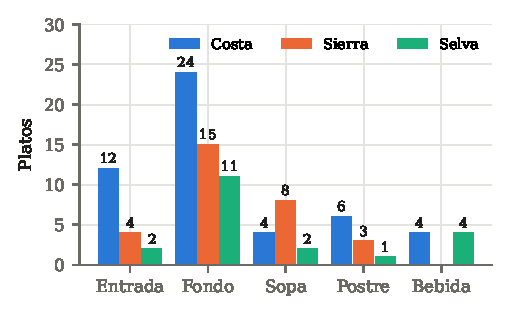
\includegraphics[width=\columnwidth]{dataset_by_type}
\caption{Platos del conjunto de datos por tipo y región.}
\label{fig:dataset}
\end{figure}

\begin{figure}[t]
\centering
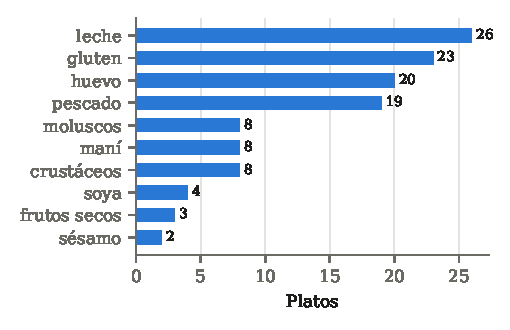
\includegraphics[width=\columnwidth]{allergen_frequency}
\caption{Número de platos que contienen cada alérgeno (incluida la contaminación cruzada), según la anotación de referencia.}
\label{fig:allergens}
\end{figure}

\begin{figure}[t]
\centering
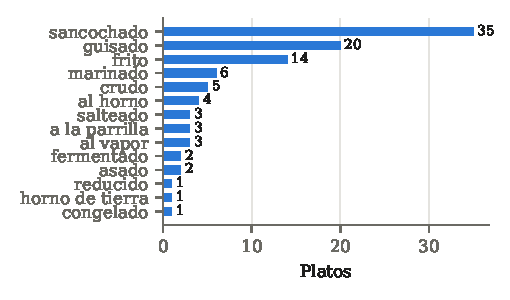
\includegraphics[width=\columnwidth]{technique_frequency}
\caption{Platos por técnica de cocción.}
\label{fig:techniques}
\end{figure}

\subsection{Modelado y construcción de la base de conocimiento}

Siguiendo METHONTOLOGY \cite{gomezperez2004}, la especificación fijó el propósito de la ontología (recomendar platos seguros y acordes con un perfil nutricional cualitativo) y sus preguntas de competencia, entre ellas: ¿qué platos de la costa no contienen crustáceos?, ¿qué platos vegetarianos no contienen leche?, ¿qué platos de Trujillo son altos en proteínas?, ¿qué ingredientes de un plato aportan un alérgeno? y ¿qué platos son aptos para la pérdida de peso y no contienen huevo? Cada consulta del banco de pruebas es una instancia de estas preguntas.

En la conceptualización, la Fig.~\ref{fig:classes} muestra las clases y propiedades principales. Las propiedades de objeto son \texttt{tieneIngrediente}, \texttt{tieneComponente} (transitiva), \texttt{sinonimoDe}, \texttt{contieneAlergeno}, \texttt{puedeContener}, \texttt{tecnicaDeCoccion} y \texttt{region} (ambas funcionales); las de datos son \texttt{ciudad}, \texttt{tipoDePlato}, \texttt{fuente}, \texttt{tipoDeAlimento} y \texttt{esTecnicaSaludable}. Se declaró la cadena de propiedades de OWL~2 \texttt{tieneIngrediente} $\circ$ \texttt{tieneComponente} $\sqsubseteq$ \texttt{tieneIngrediente}, que formaliza que un plato contiene los componentes de sus ingredientes; la clase \texttt{PlatoAptoParaPerdidaDePeso} se definió como equivalente a la intersección de \texttt{PlatoBajoEnCalorias} y \texttt{PlatoAltoEnProteinas}, y \texttt{PlatoVegano} como subclase de \texttt{PlatoVegetariano}.

\begin{figure}[t]
\centering
\resizebox{\columnwidth}{!}{%
\begin{tikzpicture}[
  cls/.style={draw, rounded corners=2pt, font=\scriptsize\ttfamily, inner sep=2.5pt, fill=blue!6, align=center},
  rel/.style={-{Stealth[length=4pt]}, font=\tiny\ttfamily},
  sub/.style={-{Triangle[open,length=5pt]}}]
\node[cls] (plato) at (0,0) {Plato};
\node[cls] (ing) at (3.6,0) {Ingrediente};
\node[cls] (alg) at (3.6,-1.7) {Alergeno};
\node[cls] (ins) at (3.6,1.4) {InsumoAndino, InsumoMarino\\InsumoAmazonico, InsumoGeneral};
\node[cls] (tec) at (-0.2,1.4) {TecnicaDeCoccion};
\node[cls] (reg) at (-2.6,0) {RegionGastronomica};
\node[cls] (perf) at (-2.4,-2.3) {PlatoBajoEnCalorias\\PlatoAltoEnProteinas\\PlatoAptoParaPerdidaDePeso\\PlatoAptoParaMantenimientoDePeso};
\node[cls] (diet) at (1.5,-2.6) {PlatoVegetariano\\PlatoVegano};
\draw[rel] (plato) -- node[above] {tieneIngrediente} (ing);
\draw[rel] (ing) -- node[right] {contieneAlergeno} (alg);
\draw[rel] (plato) -- node[above right, pos=0.55, sloped] {puedeContener} (alg);
\draw[rel] (plato) -- node[right] {tecnicaDeCoccion} (tec);
\draw[rel] (plato) -- node[above] {region} (reg);
\draw[rel] (ing.east) .. controls +(1.1,0.4) and +(1.1,-0.4) .. node[right, align=left] {tieneComponente\\sinonimoDe} (ing.east);
\draw[sub] (perf.north) -- (plato.south west);
\draw[sub] (diet.north) -- (plato.south east);
\draw[sub] (ins.south) -- (ing.north);
\end{tikzpicture}}
\caption{Clases y propiedades principales de la ontología (las flechas de punta hueca indican subclase).}
\label{fig:classes}
\end{figure}

En la implementación, la ontología terminológica (TBox) se escribió en Turtle y se pobló con un programa en Python (rdflib) que convierte cada fila del conjunto de datos en un individuo OWL. Los sinónimos se representan como individuos sin datos propios enlazados al ingrediente canónico mediante \texttt{sinonimoDe}, de modo que solo un motor que resuelva esa relación hereda los alérgenos y el tipo de alimento correspondientes. El motor de inferencia se implementó como un conjunto ordenado de reglas SPARQL Update (Tabla~\ref{tab:rules}), cuyo resultado se materializa en el grafo: la versión base aplica las reglas comunes y las de perfil base, y la versión refinada antepone las reglas de sinónimos, ingredientes derivados y contaminación cruzada y aplica las reglas de perfil refinadas. Las reglas de dietas y de perfiles usan \texttt{FILTER NOT EXISTS} sobre la lista de ingredientes, lo que implementa el supuesto de mundo cerrado que en OWL requeriría axiomas de cierre. El Listado~\ref{lst:rule} muestra la regla que materializa la cadena de propiedades.

\begin{table}[t]
\centering
\caption{Reglas de inferencia por versión}
\label{tab:rules}
\begin{tabular}{p{0.8cm}p{4.2cm}cc}
\toprule
Grupo & Regla & Base & Refinada \\
\midrule
refine & Sinónimos regionales & & \checkmark \\
refine & Ingredientes derivados (cadena) & & \checkmark \\
refine & Contaminación cruzada & & \checkmark \\
core & Alérgenos del plato & \checkmark & \checkmark \\
core & Vegetariano y vegano & \checkmark & \checkmark \\
perfil & Perfiles: técnica y categorías directas & \checkmark & \\
perfil & Perfiles: además azúcar, grasa animal, maní y frutos secos, varios lácteos, fuente proteica principal & & \checkmark \\
\bottomrule
\end{tabular}
\end{table}

\begin{lstlisting}[caption={Regla de ingredientes derivados (SPARQL Update).}, label={lst:rule}, language=SQL]
PREFIX pf: <https://thunderfruit.github.io/peruvian-food-ontology/ontology#>
INSERT { ?dish pf:tieneIngrediente ?part }
WHERE  { ?dish pf:tieneIngrediente/pf:tieneComponente+ ?part }
\end{lstlisting}

La Tabla~\ref{tab:metrics} presenta las métricas estructurales. Ambas versiones comparten 18 clases, 7 propiedades de objeto, 5 de datos y 332 individuos (100 platos, 205 ingredientes y sinónimos, 10 alérgenos, 14 técnicas y 3 regiones); difieren en los triples inferidos (2941 frente a 3115). El razonador HermiT, ejecutado mediante owlready2, clasificó ambas versiones como consistentes y sin clases insatisfacibles. La Fig.~\ref{fig:protege} muestra la versión refinada en Protégé con HermiT activo: en la jerarquía inferida, \texttt{PlatoVegetariano} queda clasificada como subclase de \texttt{Plato} y de \texttt{RestriccionAlimentaria}, y el razonador le asigna como instancias los platos que cumplen su definición.

\begin{figure}[t]
\centering
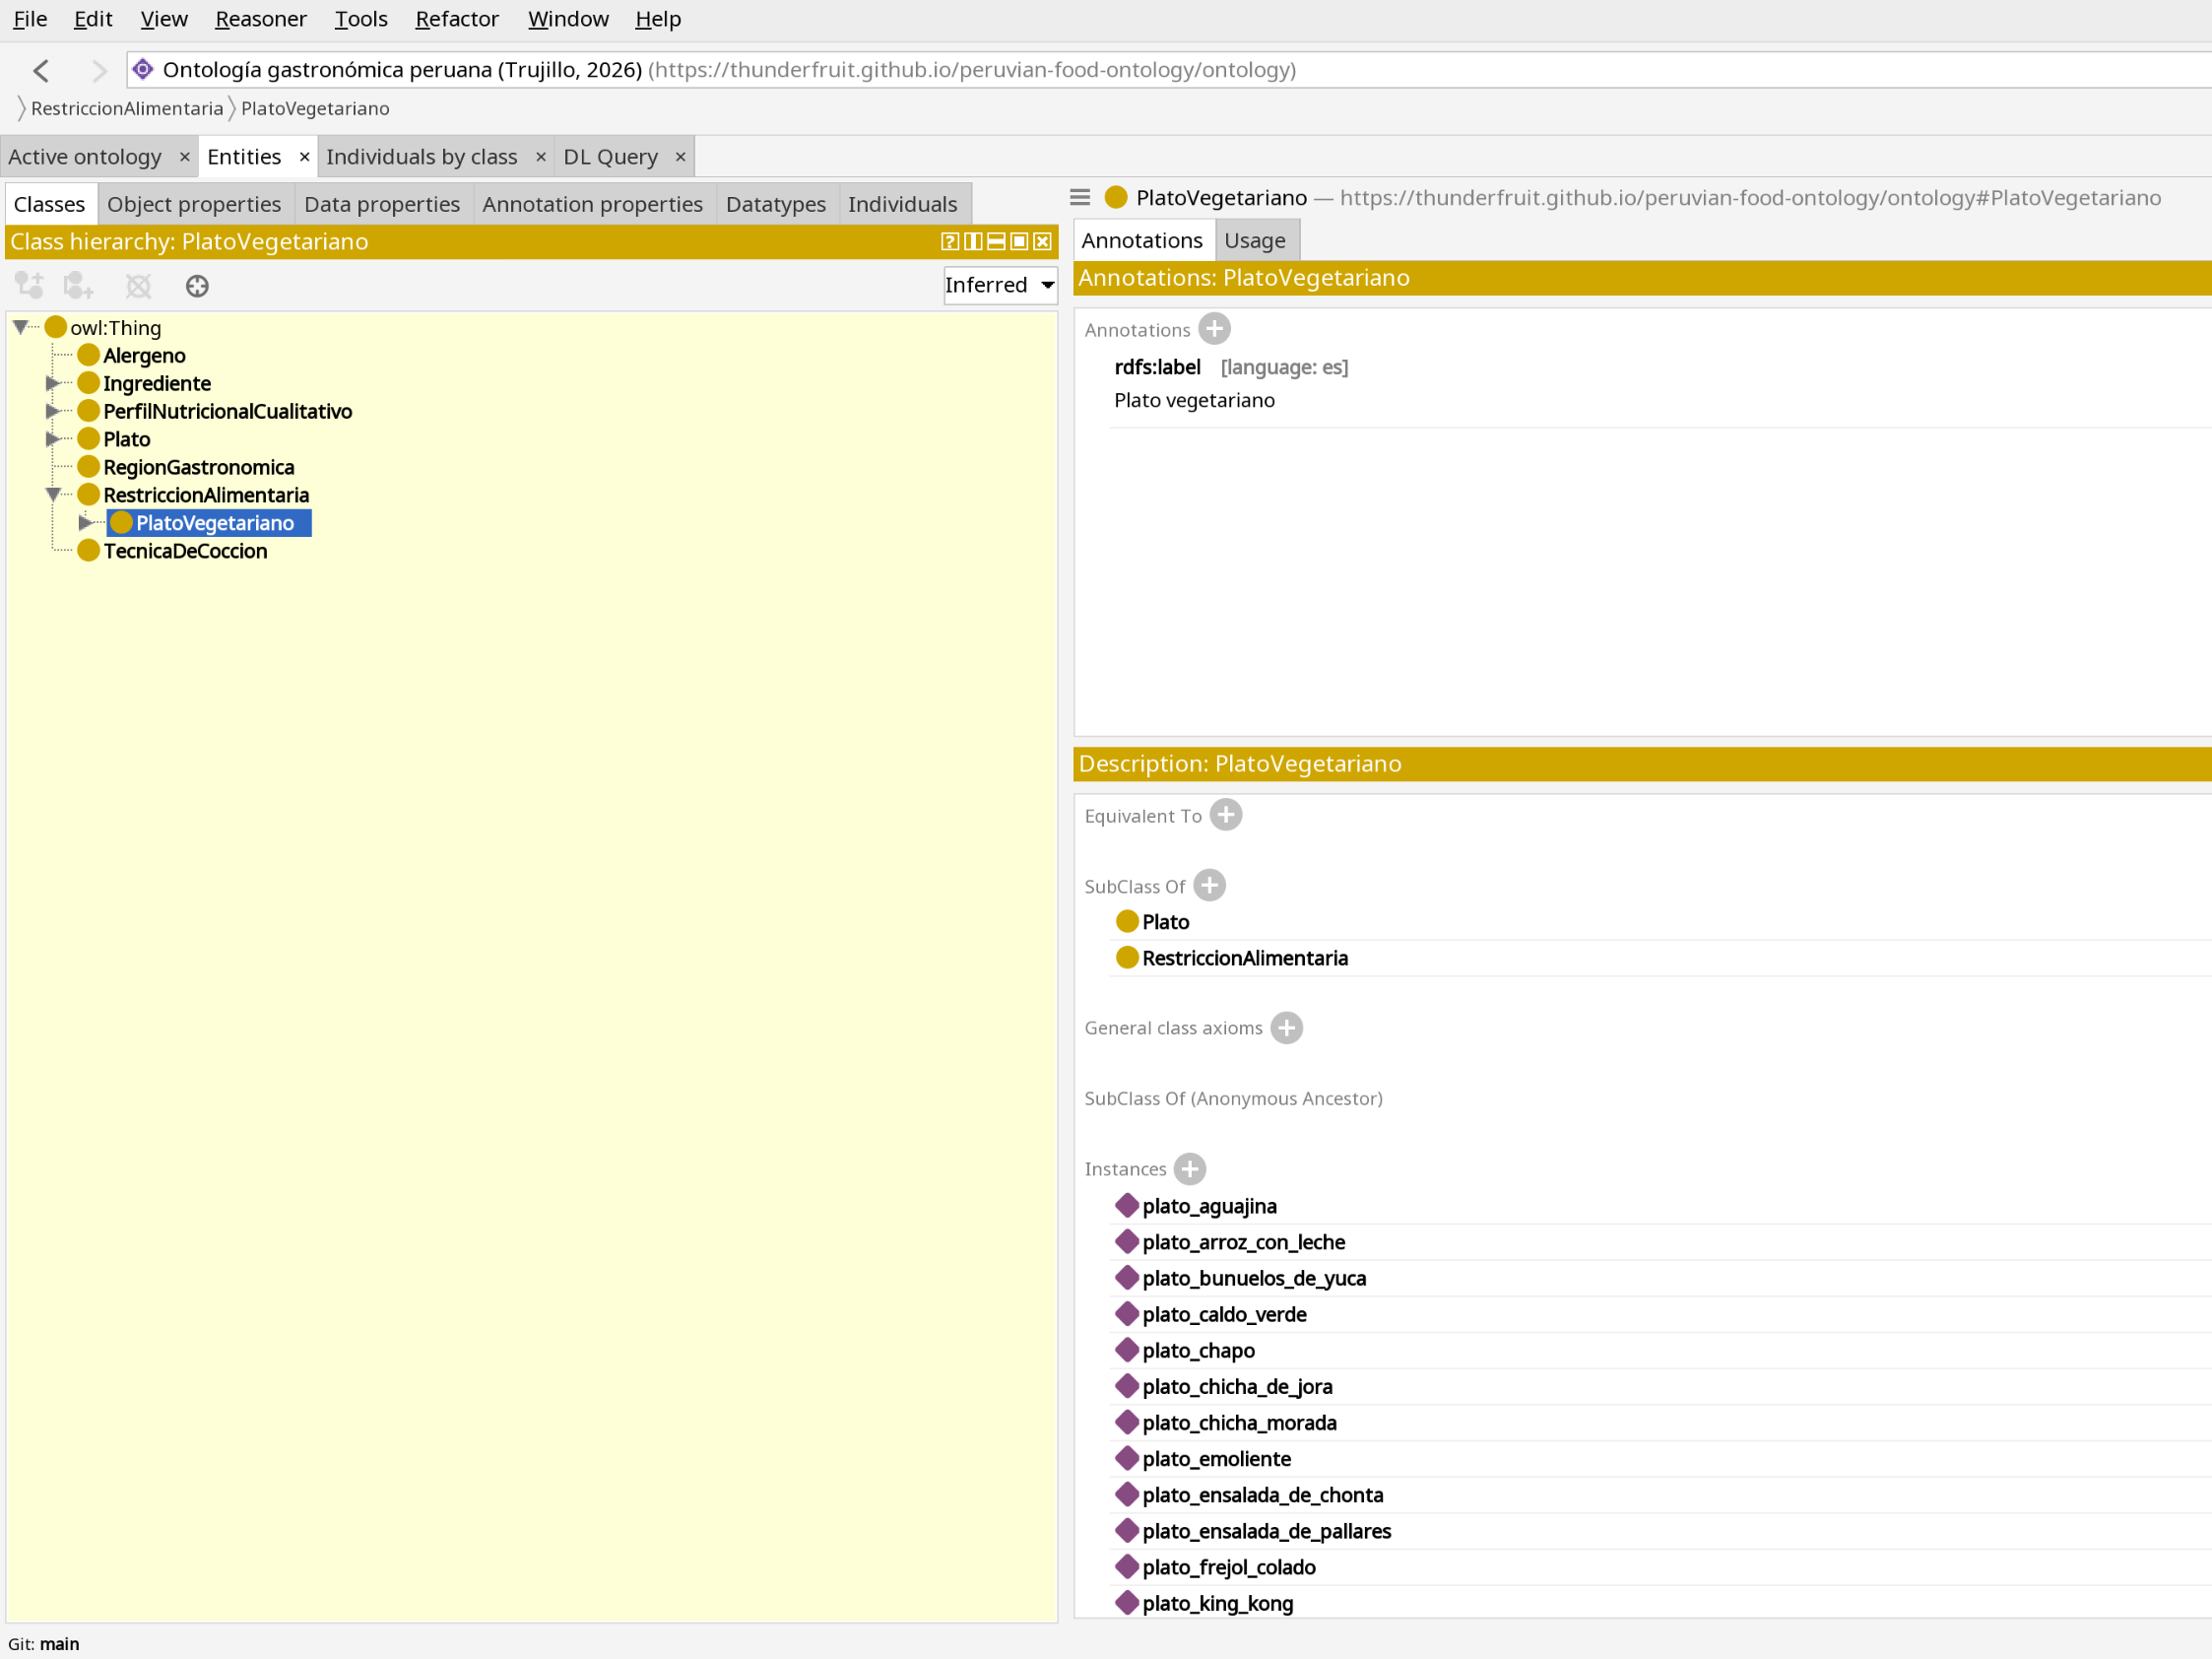
\includegraphics[width=\columnwidth]{protege_hermit}
\caption{Versión refinada de la ontología en Protégé con el razonador HermiT activo: jerarquía de clases inferida e instancias inferidas de \texttt{PlatoVegetariano}.}
\label{fig:protege}
\end{figure}

\begin{table}[t]
\centering
\caption{Métricas estructurales de la ontología}
\label{tab:metrics}
\begin{tabular}{lrr}
\toprule
Métrica & Base & Refinada \\
\midrule
Clases & 18 & 18 \\
Propiedades de objeto & 7 & 7 \\
Propiedades de datos & 5 & 5 \\
Individuos & 332 & 332 \\
Reglas de inferencia & 3 & 6 \\
Triples (tras la inferencia) & 2941 & 3115 \\
Consistencia (HermiT) & Sí & Sí \\
\bottomrule
\end{tabular}
\end{table}

\begin{figure}[t]
\centering
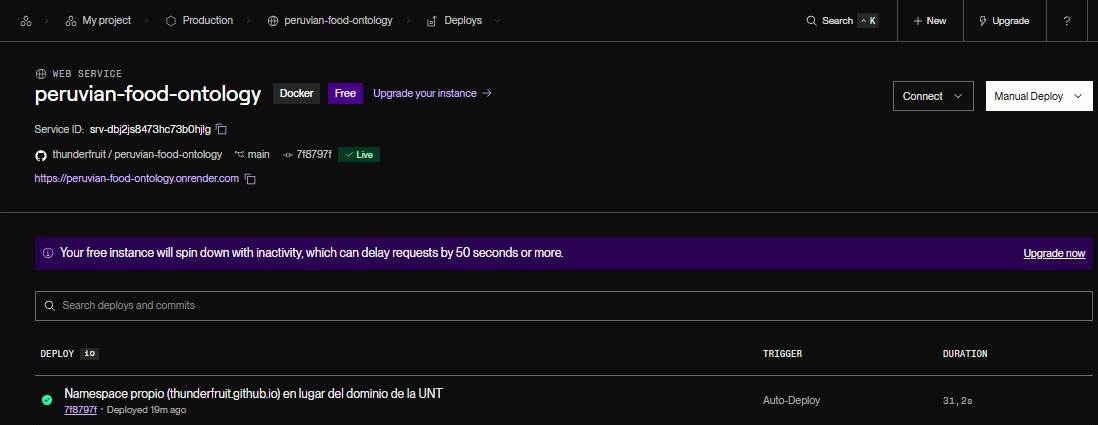
\includegraphics[width=\columnwidth]{render_service}
\caption{Servicio web en Render: imagen Docker, rama \texttt{main}, último despliegue automático (\texttt{7f8797f}) y estado \emph{Live}.}
\label{fig:render}
\end{figure}

\begin{figure}[t]
\centering
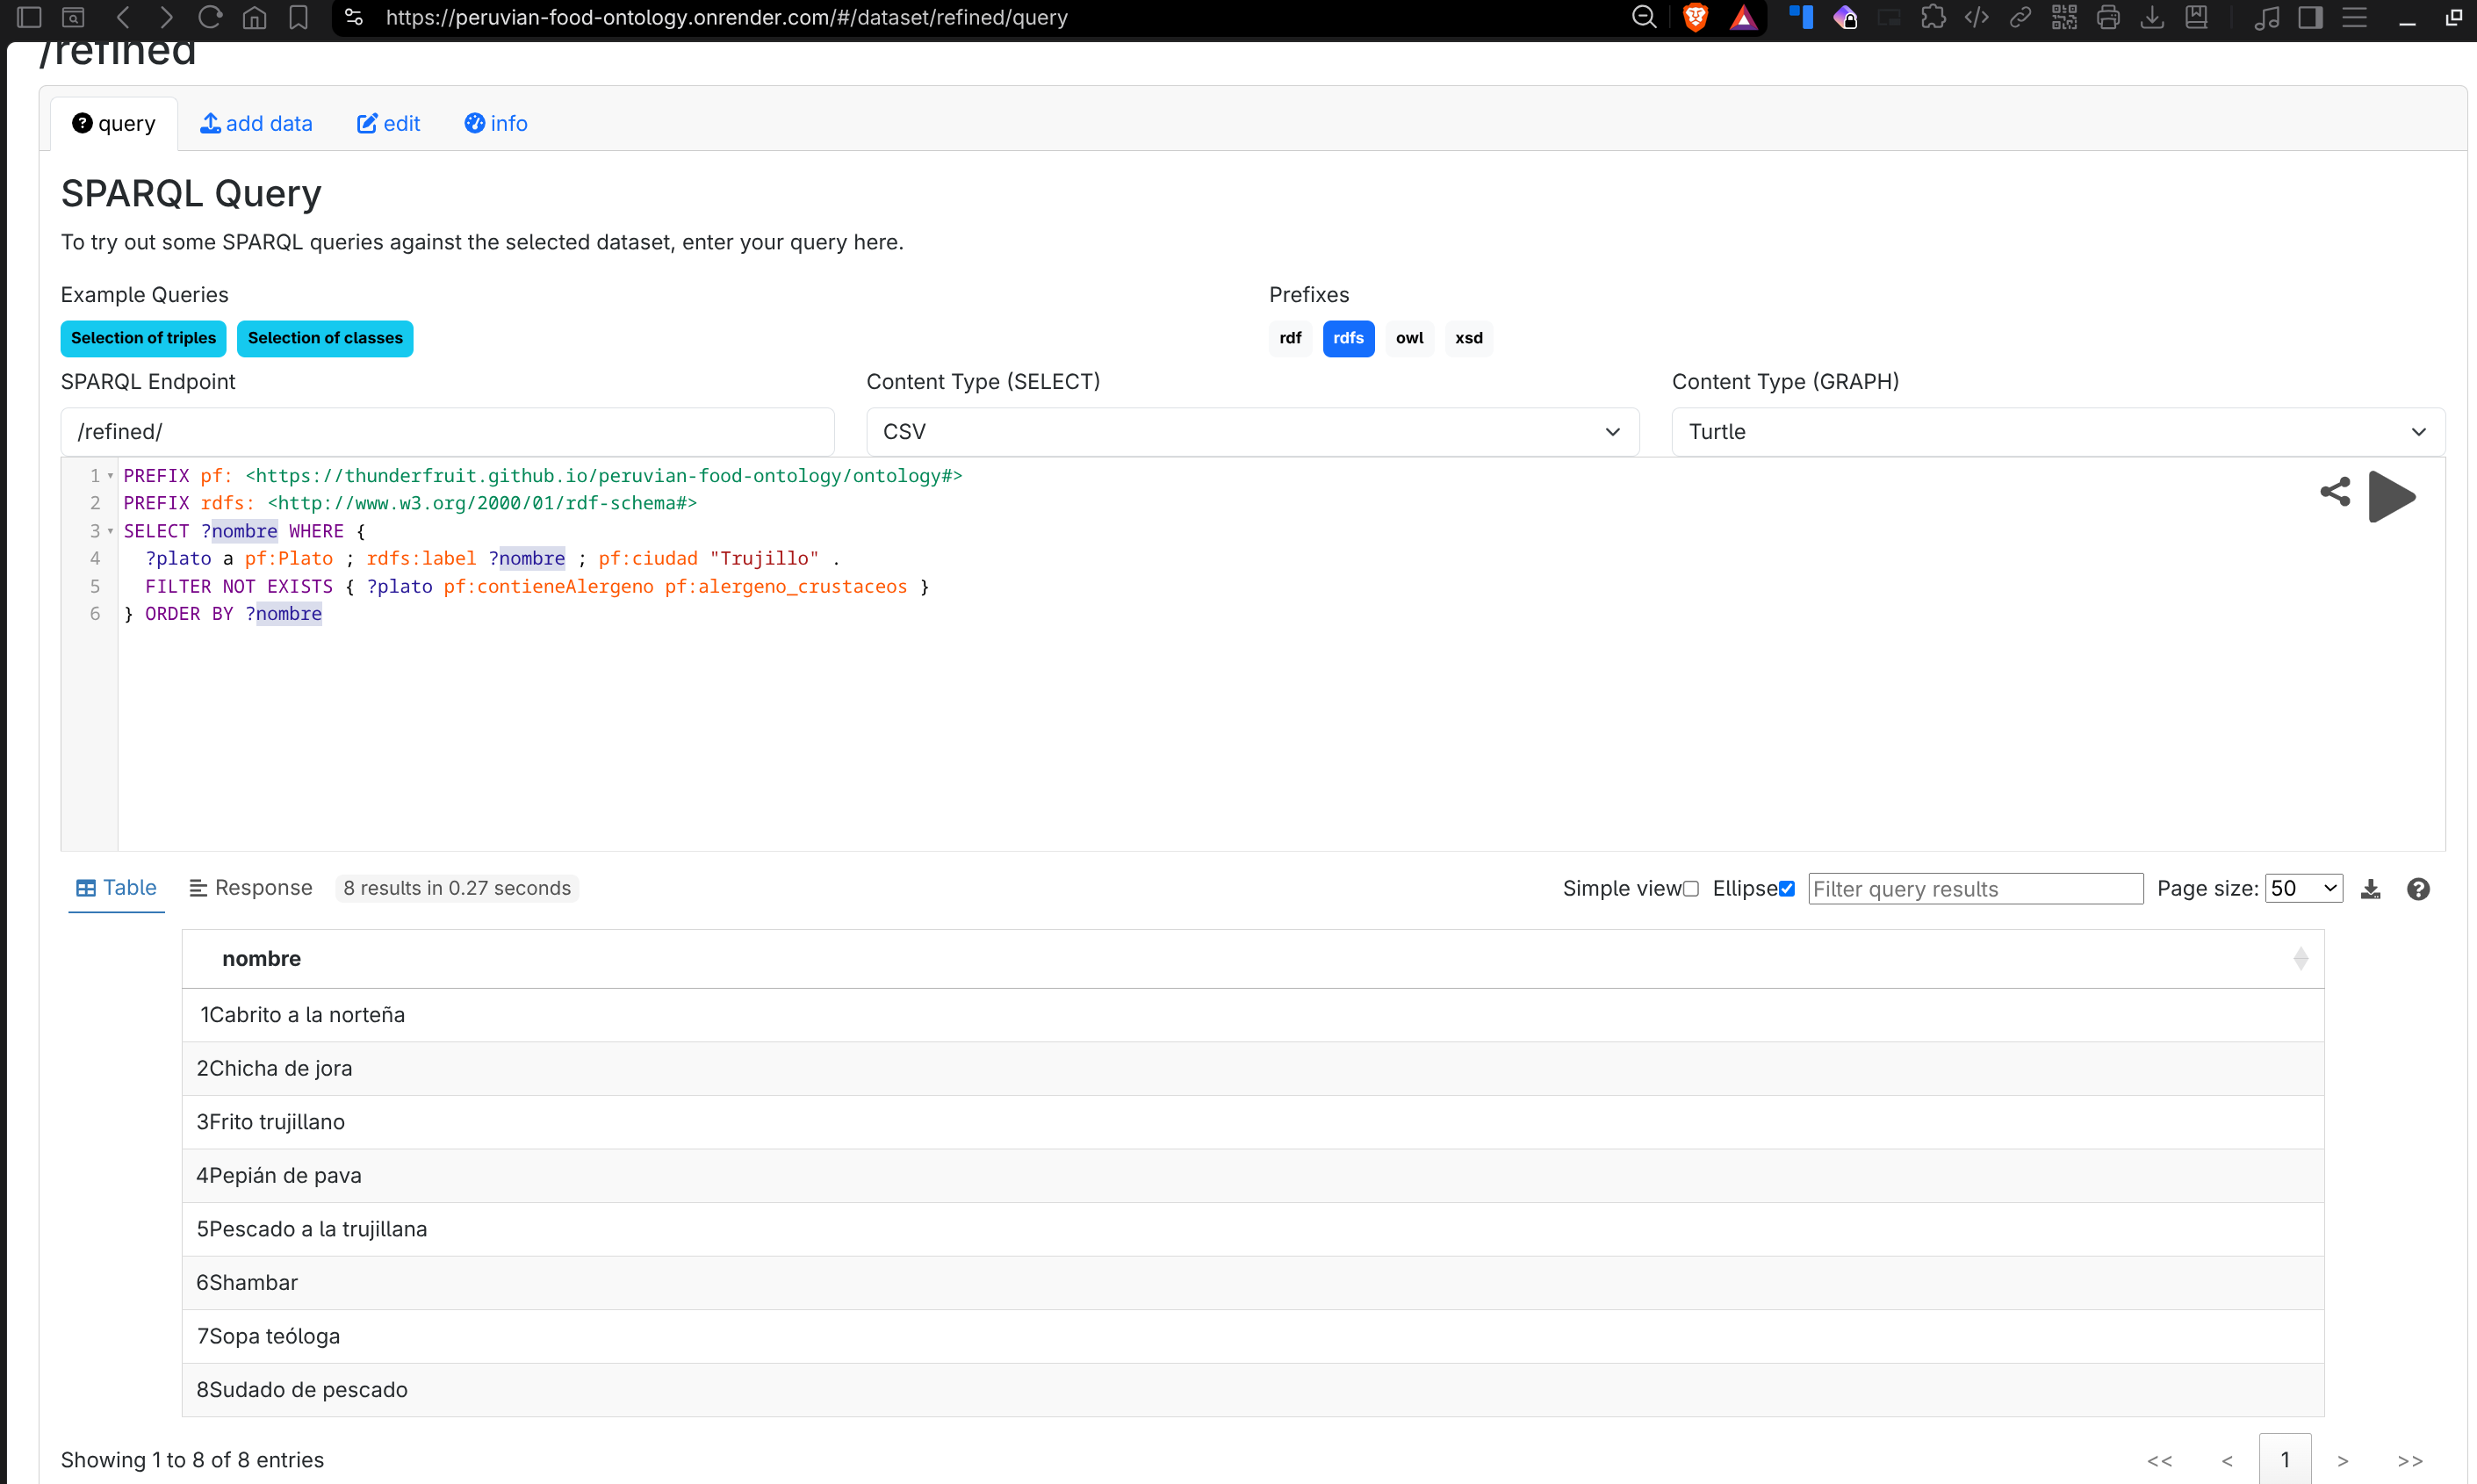
\includegraphics[width=\columnwidth]{fuseki_query}
\caption{Interfaz de Apache Jena Fuseki: consulta Q24 (platos de Trujillo sin crustáceos) sobre el servicio \texttt{/refined} desplegado en Render, con sus ocho resultados en vista de tabla.}
\label{fig:fuseki}
\end{figure}

\begin{figure*}[t]
\centering
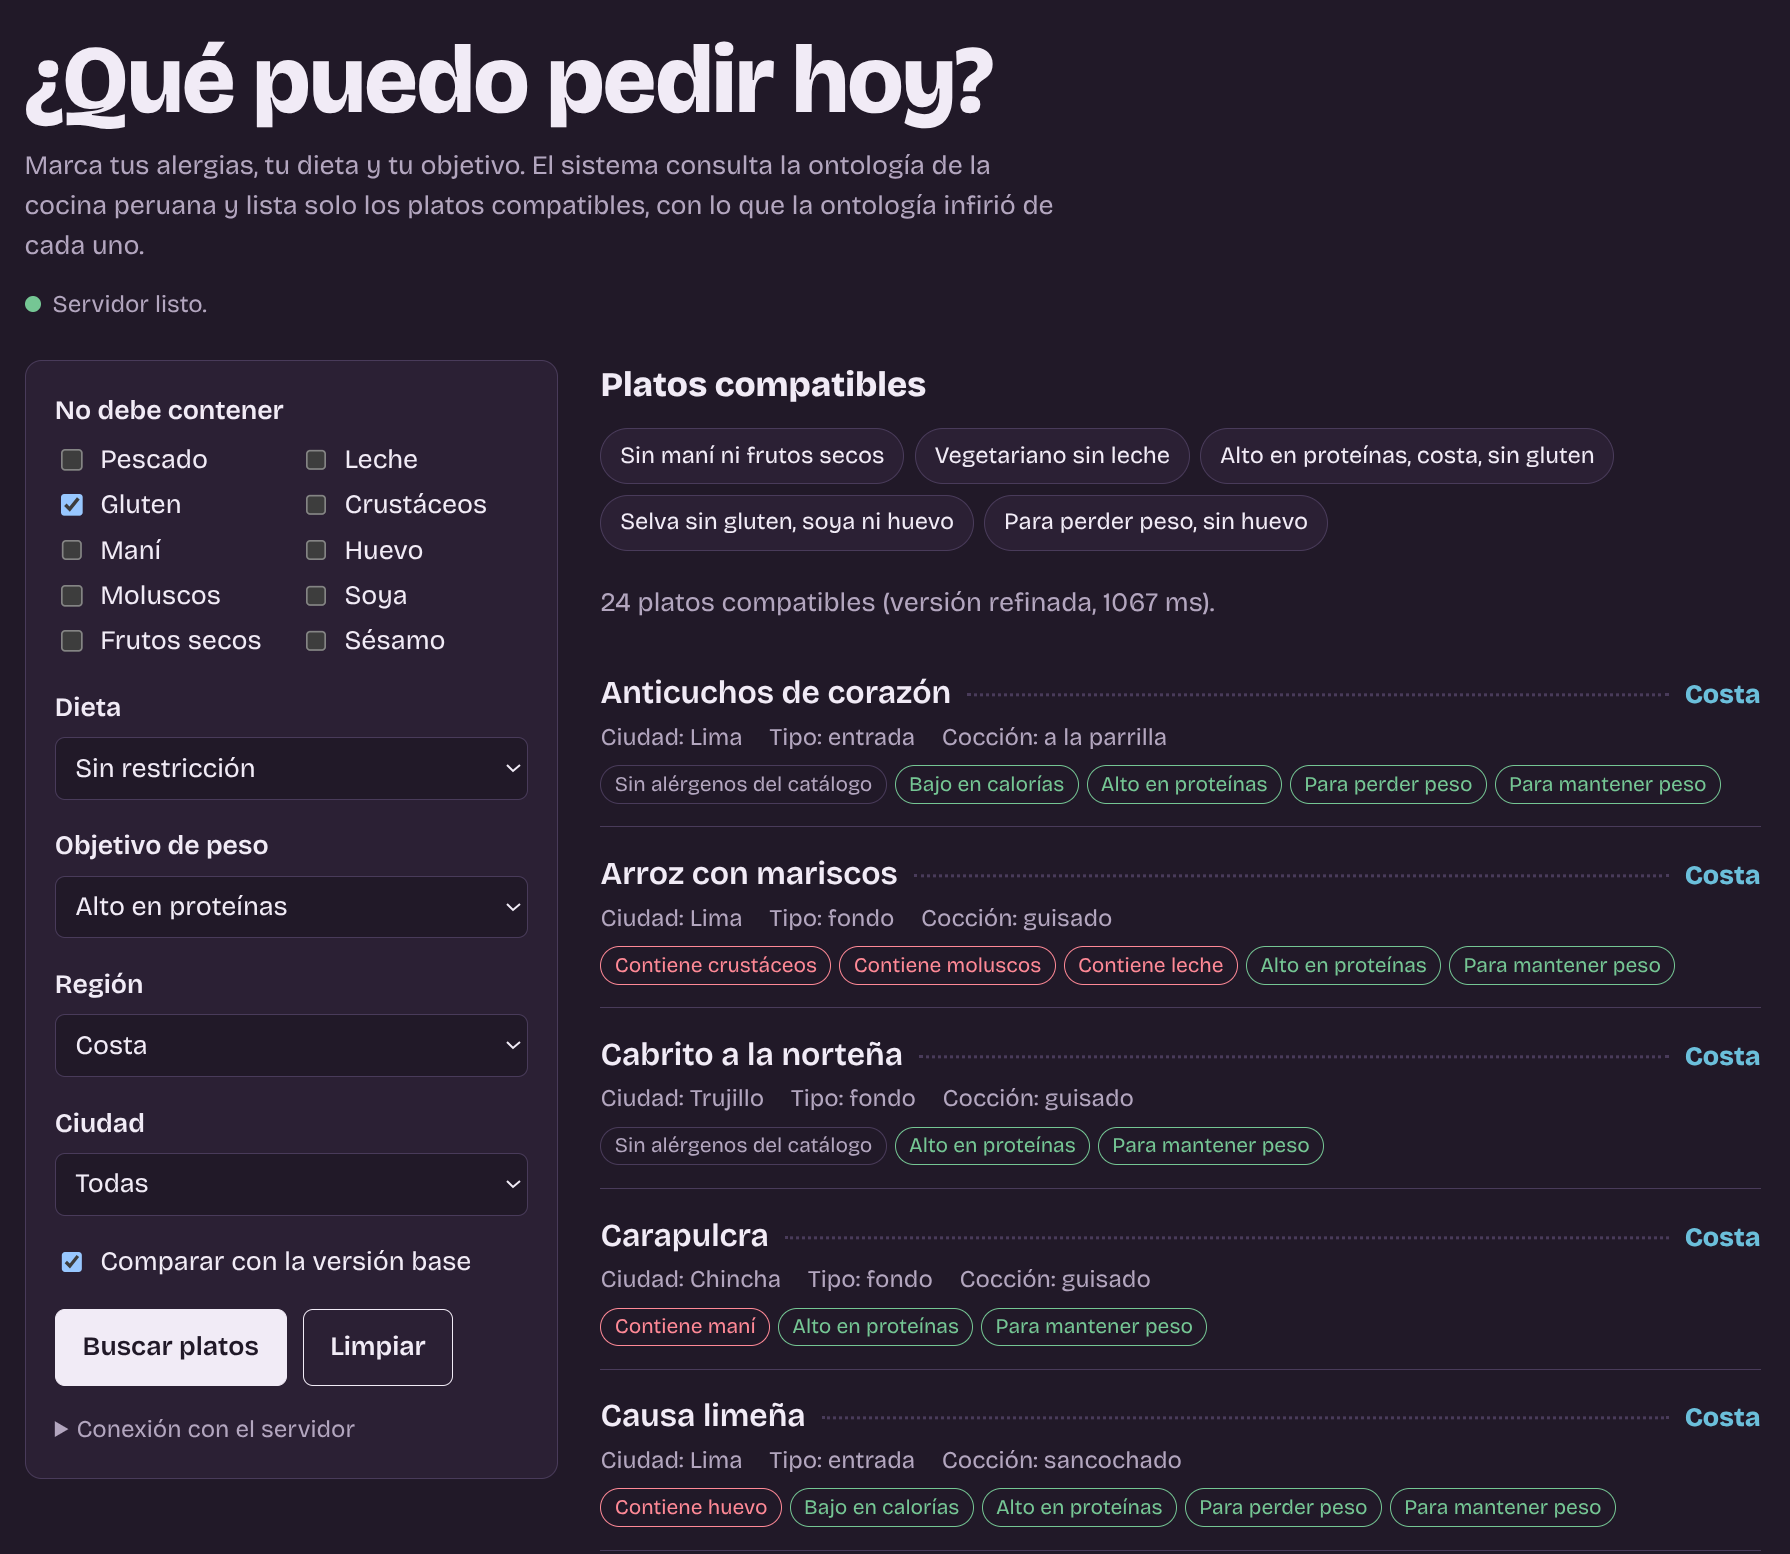
\includegraphics[height=8.2cm]{prototype_results}\hfill
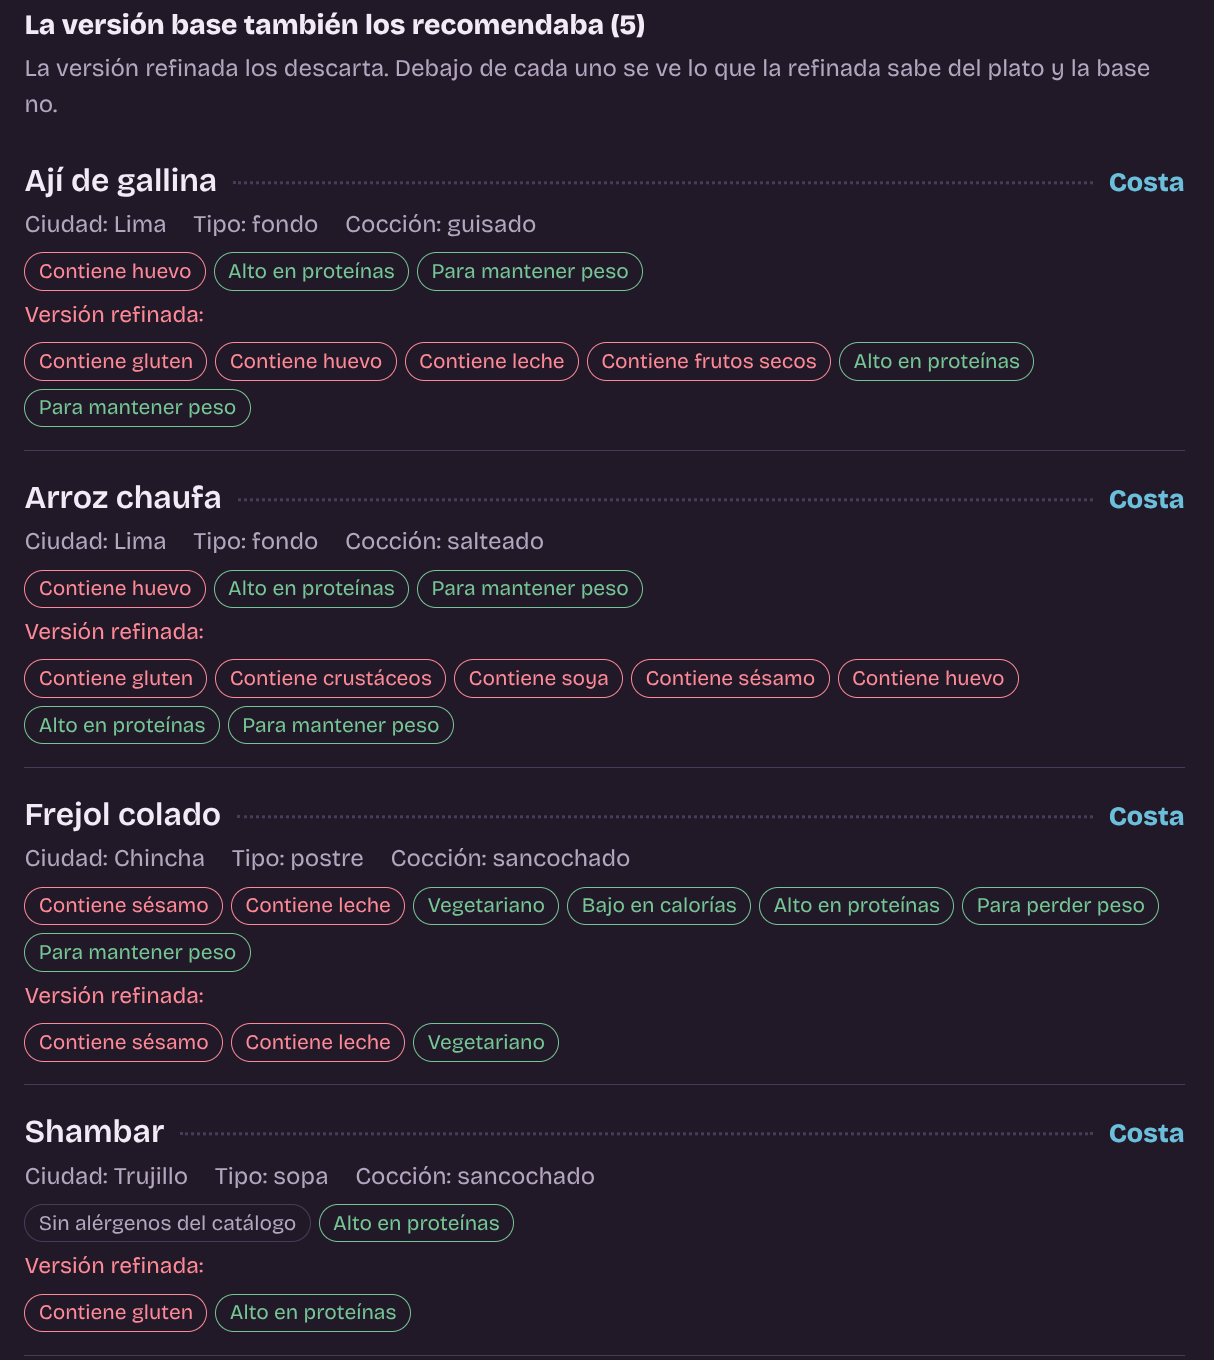
\includegraphics[height=8.2cm]{prototype_comparison}
\caption{Prototipo web con la consulta ``alto en proteínas, costa, sin gluten''. Izquierda: filtros y platos compatibles, con los alérgenos (rojo) y los perfiles inferidos (verde). Derecha: comparación con la versión base, que también recomendaba platos que la versión refinada descarta por el alérgeno que detecta.}
\label{fig:prototype}
\end{figure*}

\subsection{Despliegue en Render}

La base de conocimiento materializada de cada versión se sirve con Apache Jena Fuseki 5.2.0, empaquetado en una imagen de contenedor que incluye ambas ontologías. El archivo de configuración de Fuseki define dos servicios, \texttt{/base/query} y \texttt{/refined/query}, ambos de solo lectura, de modo que el endpoint público no admite operaciones de modificación. La imagen se despliega como servicio web en Render, que la construye directamente desde el repositorio del proyecto en cada actualización y la publica en \url{https://peruvian-food-ontology.onrender.com}. Se usó la capa gratuita, que suspende el servicio tras unos minutos sin consultas, por lo que la primera consulta después de una pausa tarda cerca de un minuto. La Fig.~\ref{fig:render} muestra el servicio desplegado, y la Fig.~\ref{fig:fuseki}, la interfaz de Fuseki ejecutando la consulta Q24 sobre la versión refinada. Antes del despliegue, el contenedor se verificó localmente: el programa de evaluación, ejecutado contra el endpoint de Fuseki, produjo exactamente las mismas métricas que contra los archivos locales, y un intento de operación de actualización fue rechazado con el código HTTP 405. Tras el despliegue, la evaluación ejecutada contra el endpoint público reprodujo las mismas métricas. El procedimiento completo se documenta en el repositorio.

Para evidenciar el uso del sistema por un consumidor, sobre el endpoint público se construyó un prototipo web (\texttt{prototype/recommender.html}), una sola página sin servidor propio, publicada en GitHub Pages (\url{https://thunderfruit.github.io/peruvian-food-ontology/prototype/recommender.html}). El usuario marca los alérgenos que debe evitar (los 10 del catálogo), elige una dieta (vegetariana o vegana), un objetivo de peso (los cuatro perfiles cualitativos) y, opcionalmente, una región o una ciudad; también dispone de cinco consultas de ejemplo que se ejecutan con un clic. Con esas opciones, el prototipo arma la consulta SPARQL: cada dieta y cada perfil se traduce en un patrón de pertenencia a la clase inferida correspondiente, y los alérgenos, en un filtro \texttt{FILTER NOT EXISTS} sobre \texttt{contieneAlergeno}. Cada plato compatible se muestra con su región, ciudad, tipo y técnica de cocción, y con lo que la ontología infirió de él: sus alérgenos y las clases de dieta y de perfil a las que pertenece, lo que hace explicable la recomendación. La consulta generada puede inspeccionarse en la misma página. Una opción de comparación ejecuta la misma consulta sobre ambas versiones y lista aparte los platos que solo la versión base recomendaba, junto con el alérgeno que la versión refinada detecta en ellos, y los platos compatibles que la versión base omitía; así, la interfaz muestra de forma directa el efecto del refinamiento medido en la evaluación. Como la capa gratuita de Render suspende el servicio, la página lo despierta al cargarse e indica su estado. Además, recuerda al usuario que confirme los ingredientes con el restaurante, porque la recomendación no reemplaza la indicación de un profesional de la salud. La Fig.~\ref{fig:prototype} muestra el prototipo con la consulta de ejemplo ``alto en proteínas, costa, sin gluten'': a la izquierda, los platos compatibles con sus etiquetas; a la derecha, los platos que solo recomendaba la versión base, como el arroz chaufa, en el que la versión refinada detecta gluten y soya por el sillao.



\subsection{Evaluación de las recomendaciones}

El programa de evaluación genera la consulta SPARQL de cada caso de prueba a partir de sus criterios, la ejecuta sobre cada versión, compara el resultado con el conjunto esperado y registra $TP$, $FP$, $FN$, $TN$, Precision, Recall y F$_1$. Las consultas son idénticas para ambas versiones; por ejemplo, la consulta Q24 (platos de Trujillo sin crustáceos) es:

\begin{lstlisting}[language=SQL]
PREFIX pf: <https://thunderfruit.github.io/peruvian-food-ontology/ontology#>
SELECT DISTINCT ?plato WHERE {
  ?plato a pf:Plato .
  ?plato pf:ciudad "Trujillo" .
  FILTER NOT EXISTS { ?plato pf:contieneAlergeno ?a .
    VALUES ?a { pf:alergeno_crustaceos } }
}
\end{lstlisting}

La Tabla~\ref{tab:results} resume los resultados sobre las 30 consultas. La versión refinada elevó la Precision media de 0,668 a 0,918, el Recall de 0,909 a 0,987 y la F$_1$ de 0,735 a 0,942, y redujo la dispersión entre consultas (desviación estándar de la F$_1$ de 0,245 a 0,124). La mejora se mantiene en los tres grupos de consultas, según su número de criterios. La Fig.~\ref{fig:precision} muestra la Precision por consulta: la versión refinada iguala o supera a la base en todas ellas.

\begin{table}[t]
\centering
\caption{Métricas medias por versión y grupo de consultas}
\label{tab:results}
\begin{tabular}{llccc}
\toprule
Grupo & Versión & Precision & Recall & F$_1$ \\
\midrule
\multirow{2}{*}{Todas (30)} & Base & 0,668 & 0,909 & 0,735 \\
 & Refinada & \textbf{0,918} & \textbf{0,987} & \textbf{0,942} \\
\midrule
\multirow{2}{*}{1 criterio (12)} & Base & 0,696 & 0,908 & 0,769 \\
 & Refinada & 0,927 & 0,978 & 0,949 \\
\multirow{2}{*}{2 criterios (12)} & Base & 0,642 & 0,892 & 0,697 \\
 & Refinada & 0,924 & 0,989 & 0,948 \\
\multirow{2}{*}{3 o más (6)} & Base & 0,664 & 0,944 & 0,742 \\
 & Refinada & 0,889 & 1,000 & 0,917 \\
\midrule
\multirow{2}{*}{Alérgenos y dietas (19)} & Base & 0,760 & 1,000 & 0,843 \\
 & Refinada & 1,000 & 1,000 & 1,000 \\
\multirow{2}{*}{Con perfil nutricional (11)} & Base & 0,509 & 0,752 & 0,549 \\
 & Refinada & 0,777 & 0,964 & 0,843 \\
\bottomrule
\end{tabular}
\end{table}

\begin{figure*}[t]
\centering
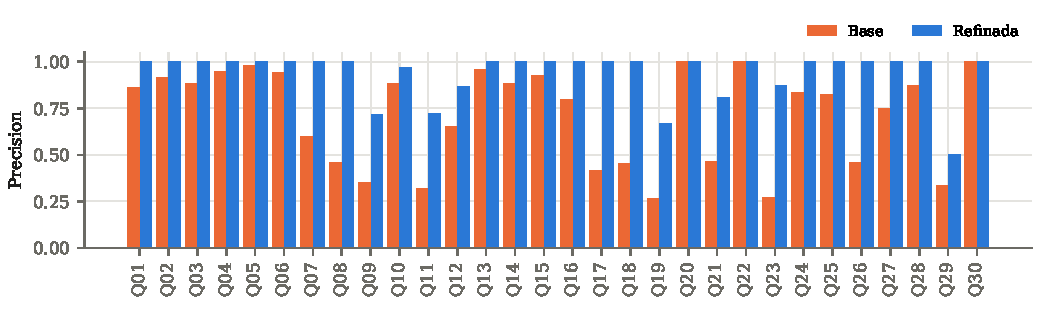
\includegraphics[width=\textwidth]{precision_by_query}
\caption{Precision por consulta en las versiones base y refinada.}
\label{fig:precision}
\end{figure*}

La Fig.~\ref{fig:confusion} presenta la matriz de confusión agregada sobre los 3000 pares consulta--plato. Los falsos positivos, que representan el error crítico en términos de seguridad, se redujeron de 400 a 45 ($-88{,}8$~\%), y los falsos negativos, de 56 a 9.

\begin{figure}[t]
\centering
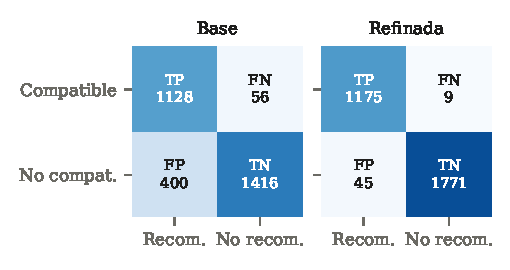
\includegraphics[width=\columnwidth]{confusion_matrices}
\caption{Matriz de confusión agregada sobre los 3000 pares consulta--plato.}
\label{fig:confusion}
\end{figure}

Para el contraste estadístico, la prueba de Shapiro--Wilk rechazó la normalidad de las diferencias por consulta en las tres métricas ($p=0{,}002$ para Precision, $p<0{,}001$ para Recall y $p=0{,}001$ para F$_1$), por lo que se aplicó la prueba de rangos con signo de Wilcoxon (Tabla~\ref{tab:stats}). Las diferencias a favor de la versión refinada son significativas en las tres métricas ($p<0{,}05$). Ninguna consulta empeoró en Precision ni en F$_1$; solo la consulta Q12 (mantenimiento de peso) perdió Recall, porque las reglas refinadas excluyen del perfil el patachi y el pato a la ucayalina, de ahí el estadístico $W=1$ en esa métrica.

\begin{table}[t]
\centering
\caption{Contraste base frente a refinada (Wilcoxon, $\alpha=0{,}05$)}
\label{tab:stats}
\begin{tabular}{lccc}
\toprule
Métrica & Shapiro--Wilk $p$ & $W$ & $p$ \\
\midrule
Precision & 0,002 & 0 & $<0{,}001$ \\
Recall & $<0{,}001$ & 1 & 0,017 \\
F$_1$ & 0,001 & 0 & $<0{,}001$ \\
\bottomrule
\end{tabular}
\end{table}

El análisis de errores explica la mejora. En la versión base, los falsos positivos de las consultas sobre alérgenos y dietas se deben a tres causas: (i) ingredientes escritos con su sinónimo regional, como el ceviche, cuyo «lenguado» no se reconocía como pescado, o el shambar, cuyo «trigo» no se reconocía como cereal con gluten; (ii) ingredientes derivados, como la papa a la huancaína, cuya salsa aporta leche, gluten y huevo; y (iii) la contaminación cruzada no considerada, como el chicharrón de pescado preparado en freidoras compartidas con mariscos. Las reglas refinadas eliminan los tres tipos de error, y las 19 consultas sobre alérgenos y dietas alcanzan Precision y Recall de 1,0. En los perfiles, la versión base clasificaba como bajos en calorías los postres y bebidas azucarados y las preparaciones con varios lácteos, y como altos en proteínas los platos con huevo o queso como acompañamiento; las reglas refinadas corrigen estos patrones. Los errores residuales (45 falsos positivos y 9 falsos negativos) se concentran en los perfiles nutricionales cualitativos de preparaciones como la causa, el chairo, el chayro, el caldo de cabeza, la patasca o el sudado de pescado, cuya clasificación depende de las porciones y de la cantidad de grasa, información que el modelo cualitativo no representa. Se optó por no añadir reglas específicas para estos platos, para no sobreajustar el motor al banco de pruebas.

\begin{thebibliography}{99}

\bibitem{bertini2026} A. Bertini, H. Cáceres-Ozimica, R. Valenzuela, and S. Durán-Agüero, ``Global and regional inequalities in dairy recommendations: A natural language processing analysis of food-based dietary guidelines across income groups,'' \emph{Lancet Reg. Health--Americas}, vol. 62, Art. no. 101550, 2026, doi: 10.1016/j.lana.2026.101550.

\bibitem{bindt2026} F. Bindt, M. Ocké, R. de Jonge, I. Toxopeus, and A. Fensel, ``NICE-Food KG: A knowledge graph for the analysis of the nutritional, ingredient, contaminant, and environmental characteristics of food for food system research,'' \emph{Future Foods}, vol. 13, Art. no. 100935, 2026, doi: 10.1016/j.fufo.2026.100935.

\bibitem{maruvada2020} P. Maruvada \emph{et al.}, ``Perspective: Dietary biomarkers of intake and exposure---Exploration with omics approaches,'' \emph{Adv. Nutr.}, vol. 11, no. 2, pp. 200--215, 2020, doi: 10.1093/advances/nmz075.

\bibitem{callahan2022} E. A. Callahan \emph{et al.}, ``Assessing the safety of bioactive ingredients in infant formula that affect the immune system: Recommendations from an expert panel,'' \emph{Am. J. Clin. Nutr.}, vol. 115, no. 2, pp. 570--587, 2022, doi: 10.1093/ajcn/nqab346.

\bibitem{spoladore2024} D. Spoladore \emph{et al.}, ``A knowledge-based decision support system for recommending safe recipes to individuals with dysphagia,'' \emph{Comput. Biol. Med.}, vol. 171, Art. no. 108193, 2024, doi: 10.1016/j.compbiomed.2024.108193.

\bibitem{prasad2026} A. Prasad, Aparna S., Bhamini R., and Veena G., ``NutritionWise: Converting nutritional labels into personalized, AI-driven nutritional insights,'' \emph{Procedia Comput. Sci.}, vol. 283, pp. 3307--3317, 2026, doi: 10.1016/j.procs.2026.06.394.

\bibitem{shafay2026} M. Shafay \emph{et al.}, ``An end-to-end vision--language framework with LLM-based reasoning for decision-oriented tomato leaf disease management in greenhouse environments,'' \emph{Comput. Electron. Agric.}, vol. 247, Art. no. 111692, 2026, doi: 10.1016/j.compag.2026.111692.

\bibitem{bagozi2026} A. Bagozi, D. Bianchini, M. Garda, M. Melchiori, and A. Rula, ``Ontology-enhanced RAG for a personalised and sustainable food advisory system,'' \emph{Data Knowl. Eng.}, vol. 164, Art. no. 102579, 2026, doi: 10.1016/j.datak.2026.102579.

\bibitem{forouzandeh2024uifrs} S. Forouzandeh, K. Berahmand, M. Rostami, A. Aminzadeh, and M. Oussalah, ``UIFRS-HAN: User interests-aware food recommender system based on the heterogeneous attention network,'' \emph{Eng. Appl. Artif. Intell.}, vol. 135, Art. no. 108766, 2024, doi: 10.1016/j.engappai.2024.108766.

\bibitem{forouzandeh2024health} S. Forouzandeh, M. Rostami, K. Berahmand, and R. Sheikhpour, ``Health-aware food recommendation system with dual attention in heterogeneous graphs,'' \emph{Comput. Biol. Med.}, vol. 169, Art. no. 107882, 2024, doi: 10.1016/j.compbiomed.2023.107882.

\bibitem{asani2021} E. Asani, H. Vahdat-Nejad, and J. Sadri, ``Restaurant recommender system based on sentiment analysis,'' \emph{Mach. Learn. Appl.}, vol. 6, Art. no. 100114, 2021, doi: 10.1016/j.mlwa.2021.100114.

\bibitem{garcia2025} I. X. García del Moral Lara, ``La inteligencia artificial en la elaboración de recetas de cocina: Fortaleciendo la identidad culinaria de Quintana Roo, México,'' \emph{Cienc. Lat. Rev. Cient. Multidiscip.}, vol. 9, no. 2, pp. 3209--3238, abr. 2025, doi: 10.37811/cl\_rcm.v9i2.17134.

\bibitem{jonquet2018} C. Jonquet \emph{et al.}, ``AgroPortal: A vocabulary and ontology repository for agronomy,'' \emph{Comput. Electron. Agric.}, vol. 144, pp. 126--143, 2018, doi: 10.1016/j.compag.2017.10.012.

\bibitem{urdu2024} D. Urdu \emph{et al.}, ``Aligning interoperability architectures for digital agri-food platforms,'' \emph{Comput. Electron. Agric.}, vol. 224, Art. no. 109194, 2024, doi: 10.1016/j.compag.2024.109194.

\bibitem{gomezperez2004} A. Gómez-Pérez, M. Fernández-López, and O. Corcho, \emph{Ontological Engineering: With Examples from the Areas of Knowledge Management, e-Commerce and the Semantic Web}. London, U.K.: Springer, 2004.

\bibitem{allemang2008} D. Allemang and J. Hendler, \emph{Semantic Web for the Working Ontologist: Modeling in RDF, RDFS and OWL}. Burlington, MA, USA: Morgan Kaufmann, 2008.

\bibitem{sanchez2025} J.-M. Sánchez-Martín, R. Guillén-Peñafiel, and A.-M. Hernández-Carretero, ``Artificial intelligence in heritage tourism: Innovation, accessibility, and sustainability in the digital age,'' \emph{Heritage}, vol. 8, no. 10, Art. no. 428, 2025, doi: 10.3390/heritage8100428.

\bibitem{li2020} J. Li, B. Maharjan, B. Xie, and C. Tao, ``A personalized voice-based diet assistant for caregivers of Alzheimer disease and related dementias: System development and validation,'' \emph{J. Med. Internet Res.}, vol. 22, no. 9, 2020, doi: 10.2196/19897.

\bibitem{xu2024} Z. Xu \emph{et al.}, ``Developing a personalized meal recommendation system for Chinese older adults: Observational cohort study,'' \emph{JMIR Form. Res.}, vol. 8, 2024, doi: 10.2196/52170.

\bibitem{sha2025} H. Sha, F. Gong, B. Liu, R. Liu, H. Wang, and T. Wu, ``Leveraging retrieval-augmented large language models for dietary recommendations with Traditional Chinese Medicine's medicine food homology: Algorithm development and validation,'' \emph{JMIR Med. Inform.}, vol. 13, 2025, doi: 10.2196/75279.

\bibitem{hitzler2009} P. Hitzler, M. Krötzsch, and S. Rudolph, \emph{Foundations of Semantic Web Technologies}. Boca Raton, FL, USA: Chapman and Hall/CRC, 2009.

\bibitem{un2015agenda} United Nations General Assembly, ``Transforming our world: The 2030 Agenda for Sustainable Development,'' Resolution A/RES/70/1, Oct. 2015. [Online]. Available: \url{https://sdgs.un.org/2030agenda}

\bibitem{un2024sdg3} United Nations, ``Goal 3: Ensure healthy lives and promote well-being for all at all ages,'' Department of Economic and Social Affairs, Sustainable Development. [Online]. Available: \url{https://sdgs.un.org/goals/goal3}

\bibitem{inei2012} Instituto Nacional de Estadística e Informática, ``Platos típicos regionales,'' cap. 3 en \emph{Perú: Consumo per cápita de los principales alimentos 2008--2009}. Lima, Perú: INEI, may. 2012, pp. 85--117. [Online]. Available: \url{https://www.inei.gob.pe/media/MenuRecursivo/publicaciones_digitales/Est/Lib1028/cap03.pdf}

\bibitem{andina2023} Agencia Peruana de Noticias Andina, ``Expo Amazónica 2023: deléitate con estos manjares emblemáticos de la selva peruana,'' 22 sep. 2023. [Online]. Available: \url{https://andina.pe/agencia/noticia-expo-amazonica-2023-deleitate-estos-manjares-emblematicos-de-selva-peruana-956148.aspx}

\bibitem{promperu} Comisión de Promoción del Perú para la Exportación y el Turismo (PromPerú), ``Gastronomía,'' Perú: Viaja y Descubre. [Online]. Available: \url{https://www.peru.travel}

\bibitem{palma2008} J. T. Palma Méndez and R. Marín Morales, Eds., \emph{Inteligencia Artificial: Técnicas, métodos y aplicaciones}. Madrid, España: McGraw-Hill, 2008.

\bibitem{codex2024} Codex Alimentarius Commission, ``General Standard for the Labelling of Prepackaged Foods,'' CXS 1-1985, rev. 2024. Rome, Italy: FAO/WHO.

\bibitem{marcaperu2018trujillo} Marca Perú, ``Los 5 platos típicos de Trujillo más populares,'' peru.info, 27 dic. 2018. [Online]. Available: \url{https://peru.info/es-pe/gastronomia/blogperu/2/13/los-5-platos-tipicos-de-trujillo-mas-populares}

\bibitem{andina2024trujillo} Agencia Peruana de Noticias Andina, ``¡Trujillo está de moda! Saborea y disfruta sus platos embajadores que deleitan paladares,'' 29 sep. 2024. [Online]. Available: \url{https://andina.pe/agencia/noticia-trujillo-esta-moda-saborea-y-disfruta-sus-platos-embajadores-deleitan-paladares-1001686.aspx}

\end{thebibliography}

\end{document}
